\section{eo\-Parameter\-Loader Class Reference}
\label{classeo_parameter_loader}\index{eoParameterLoader@{eoParameterLoader}}
Parameter saving and loading.  


{\tt \#include $<$eo\-Parser.h$>$}

Inheritance diagram for eo\-Parameter\-Loader::\begin{figure}[H]
\begin{center}
\leavevmode
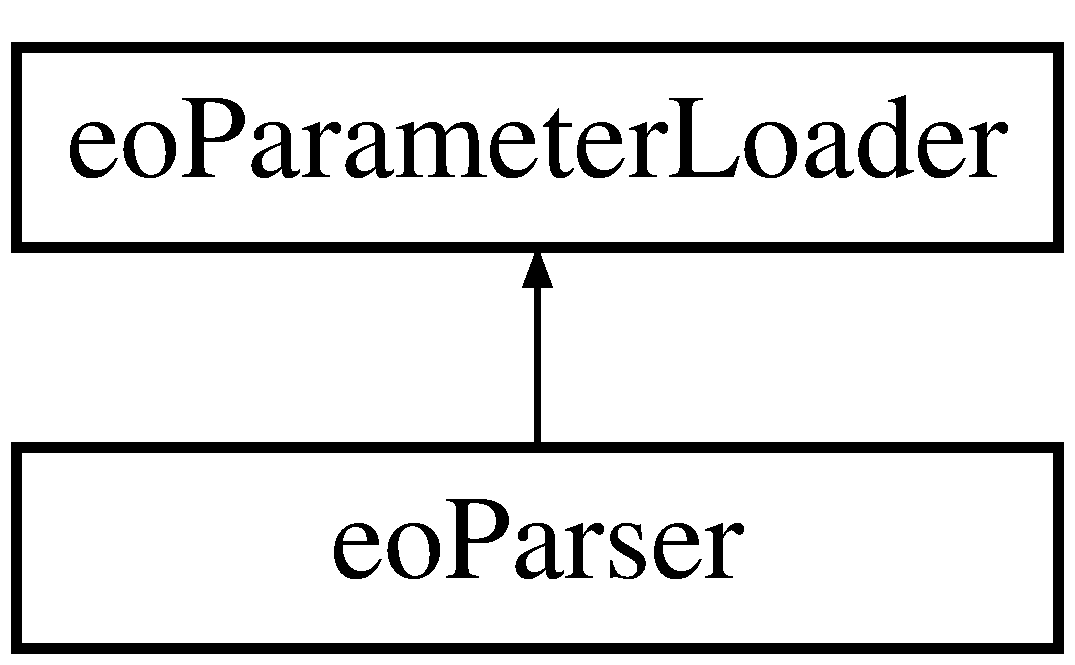
\includegraphics[height=2cm]{classeo_parameter_loader}
\end{center}
\end{figure}
\subsection*{Public Member Functions}
\begin{CompactItemize}
\item 
virtual {\bf $\sim$eo\-Parameter\-Loader} ()\label{classeo_parameter_loader_a0}

\begin{CompactList}\small\item\em Need a virtual destructor. \item\end{CompactList}\item 
virtual void {\bf process\-Param} ({\bf eo\-Param} \&param, std::string section=\char`\"{}\char`\"{})=0
\begin{CompactList}\small\item\em Register a parameter and set its value if it is known. \item\end{CompactList}\item 
virtual bool {\bf is\-It\-There} ({\bf eo\-Param} \&\_\-param) const =0\label{classeo_parameter_loader_a2}

\begin{CompactList}\small\item\em checks if \_\-param has been actually entered \item\end{CompactList}\item 
template$<$class Value\-Type$>$ {\bf eo\-Value\-Param}$<$ Value\-Type $>$ \& {\bf create\-Param} (Value\-Type \_\-default\-Value, std::string \_\-long\-Name, std::string \_\-description, char \_\-short\-Hand=0, std::string \_\-section=\char`\"{}\char`\"{}, bool \_\-required=false)
\begin{CompactList}\small\item\em Construct a Param and sets its value. \item\end{CompactList}\end{CompactItemize}
\subsection*{Private Attributes}
\begin{CompactItemize}
\item 
std::vector$<$ {\bf eo\-Param} $\ast$ $>$ {\bf owned\-Params}\label{classeo_parameter_loader_r0}

\end{CompactItemize}


\subsection{Detailed Description}
Parameter saving and loading. 

eo\-Parameter\-Loader is an abstract class that can be used as a base for your own parameter loading and saving. The command line parser {\bf eo\-Parser}{\rm (p.\,\pageref{classeo_parser})} is derived from this class. 



Definition at line 40 of file eo\-Parser.h.

\subsection{Member Function Documentation}
\index{eoParameterLoader@{eo\-Parameter\-Loader}!processParam@{processParam}}
\index{processParam@{processParam}!eoParameterLoader@{eo\-Parameter\-Loader}}
\subsubsection{\setlength{\rightskip}{0pt plus 5cm}virtual void eo\-Parameter\-Loader::process\-Param ({\bf eo\-Param} \& {\em param}, std::string {\em section} = {\tt \char`\"{}\char`\"{}})\hspace{0.3cm}{\tt  [pure virtual]}}\label{classeo_parameter_loader_a1}


Register a parameter and set its value if it is known. 

\begin{Desc}
\item[Parameters:]
\begin{description}
\item[{\em param}]the parameter to process \item[{\em section}]the section where this parameter belongs \end{description}
\end{Desc}


Implemented in {\bf eo\-Parser} {\rm (p.\,\pageref{classeo_parser_a1})}.\index{eoParameterLoader@{eo\-Parameter\-Loader}!createParam@{createParam}}
\index{createParam@{createParam}!eoParameterLoader@{eo\-Parameter\-Loader}}
\subsubsection{\setlength{\rightskip}{0pt plus 5cm}template$<$class Value\-Type$>$ {\bf eo\-Value\-Param}$<$Value\-Type$>$\& eo\-Parameter\-Loader::create\-Param (Value\-Type {\em \_\-default\-Value}, std::string {\em \_\-long\-Name}, std::string {\em \_\-description}, char {\em \_\-short\-Hand} = {\tt 0}, std::string {\em \_\-section} = {\tt \char`\"{}\char`\"{}}, bool {\em \_\-required} = {\tt false})\hspace{0.3cm}{\tt  [inline]}}\label{classeo_parameter_loader_a3}


Construct a Param and sets its value. 

The loader will own the memory thus created

\begin{Desc}
\item[Parameters:]
\begin{description}
\item[{\em \_\-default\-Value}]The default value \item[{\em \_\-long\-Name}]Long name of the argument \item[{\em \_\-description}]Description of the parameter. What is useful for. \item[{\em \_\-short\-Name}]Short name of the argument (Optional) \item[{\em \_\-section}]Name of the section where the parameter belongs \item[{\em \_\-required}]If it is a necessary parameter or not \end{description}
\end{Desc}


Definition at line 70 of file eo\-Parser.h.

Referenced by eo\-Parser::get\-ORcreate\-Param(), and eo\-Parser::set\-ORcreate\-Param().

The documentation for this class was generated from the following files:\begin{CompactItemize}
\item 
eo\-Parser.h\item 
eo\-Parser.cpp\end{CompactItemize}
